\chapter{Introdução}

\begin{flushright}
\begin{minipage}[t][0cm][b]{0.47\textwidth}
\emph{Se não podes entender, crê para que entendas. A fé precede, o intelecto segue.}
\end{minipage}

\rule[0cm]{7cm}{0.03cm}%{largura}{espessura}

Santo Agostinho
\end{flushright}


\section{Motivação e Objetivos}

Um grafo EPG $G$ é um grafo que admite uma representação em que seus vértices são representados por caminhos de uma grade $Q$, tal que dois vertices de $G$ são adjacentes se e somente se os caminhos correspondestes tem no mínimo uma aresta em comum.

Apesar dos problemas da teoria de grafos serem algumas vezes artificiais, é possível encontrar alguns problemas com motivação prática. O estudo de grafos EPG tem motivação relacionada com o problema de \textit{design} VLSI que combina a noção de grafos de intersecção de arestas de caminhos em uma árvore com um modelo de \textit{layout} de grade VLSI~\cite{golumbic2009}. O número de dobras em um circuito integrado pode aumentar a área de \textit{layout} e consequentemente aumentar o custo de produção do microchip. 
Essa é uma das principais aplicações que instigam pesquisa sobre representações EPG de algumas famílias de grafos quando existem restrições no número de dobras nos caminhos usados na representação.
Outras aplicações e detalhes sobre problemas de \textit{layout} de circuitos podem ser encontrados em~\cite{bandy1990, molitor1991}.   

Um grafo é $ B_k$-EPG se ele admite uma representação em que cada caminho possua no máximo $k$ dobras. A título de exemplo a Figura~\ref{fig:trianguloepgRepresentacao}(a) retrata um grafo $C_3$, a Figura~\ref{fig:trianguloepgRepresentacao}(b) retrata uma representação EPG onde os caminhos não possuem dobra e a  Figura~\ref{fig:trianguloepgRepresentacao}(c) retrata uma representação com 1 dobra. Consequentemente, $C_3$ é um grafo  $B_0$-EPG. De forma mais geral, grafos $B_0$-EPG coincidem com grafos de intervalo~\cite{golumbic2009}.

O \emph{bend number} de uma classe de grafos é o menor  $k$ para o qual todos os grafos na classe possuem uma representação $B_k$-EPG. Grafos de intervalor possuem bend number $0$~\cite{golumbic2009}, árvores possuem  bend number $1$~\cite{golumbic2009} e  grafos outerplanar possuem bend number $2$~\cite{daniel2014b}. O bend number para a classe dos grafos planares é um problema em aberto, porém sabe-se que ele é $ 3 $ ou $4$~\cite{daniel2014b}. %Apesar de existirem demonstrações de que o bend number não é maior que 4 para a classe dos grafos planares, também não se conhece algum grafo planar que não possa ser representado com 3 dobras.

A classe dos grafos EPG tem sido estudada em diversos trabalhos, tal como  \cite{alcon2016, Asinowski2009, cohen2014, golumbic2009, heldt2014,  martin2017}, entre outros. As investigações frequentemente abordam caracterizações com relação número de dobras das representações de um grafo. A respeito da complexidade de reconhecimento de grafos $B_k$-EPG, somente a complexidade de reconhecimento de três sub-classes de grafos EPG foi determinada:
 grafos $B_0$-EPG podem ser reconhecidos em tempo polinomial, uma vez que correspondem a classe de grafos de intervalo, ver~\cite{booth1976}. Em contraste, o reconhecimento das classes $B_1$-EPG e $B_2$-EPG é $NP$-completo, ver~\cite{heldt2014, martin2017}.

\begin{figure}[h]
  \centering
  \begin{tabular}{ c p{0.15cm} c p{0.15cm} c }
    %\centering
    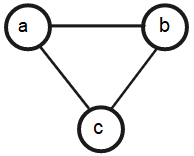
\includegraphics[width=2.3cm]{./img/trianguloabc.png} && 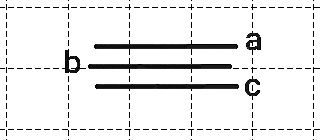
\includegraphics[width=3.5cm]{./img/b0epgTransparenciaGrade2.png} & &
    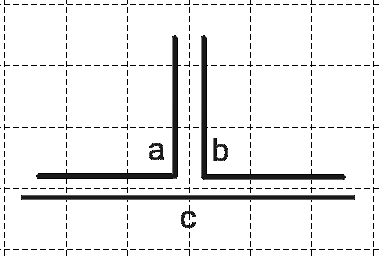
\includegraphics[width=3.5cm]{./img/b1EpgTransparenteGrade2.png}
    \\
    \footnotesize %\centering 
    (a) O grafo $C_3$ && \footnotesize(b) Representação $B_0$-EPG de $C_3$ && \footnotesize (c) Representação $B_1$-EPG de $C_3$\\

  \end{tabular}

 \caption{o grafo $ C_3 $ com duas representações, uma sem dobra e outra com uma dobra} \label{fig:trianguloepgRepresentacao}
\end{figure}


%A  collection $C$ of sets satisfies the Helly property when every sub-collection of $ C $ that is pairwise intersecting has at least one common element. The Helly property has this name in honor of the great Austrian mathematician Eduard Helly, who in 1923 proposed his famous theorem concerning the relation of intersecting sets.

%The study of the Helly property is useful in very diverse areas of science, and we can enumerate applications in semantics, code theory, computational biology, database, image processing, graph theory, optimization, and linear programming \cite{dourado2009}.

%Note that the representation of Figure~\ref{fig:trianguloepgRepresentacao}(b) satisfies the Helly property, while the representations of Figures~\ref{fig:trianguloepgRepresentacao}(c) and~\ref{fig:trianguloepgRepresentacao}(d) do not satisfy it.

Este trabalho propõe o estudo de grafos que possuam uma representação EPG-Helly. 
A propriedade Helly relacionada com representações EPG tem sido estudada por~\cite{golumbic2009} e \cite{golumbic2013}. Em particular, esses trabalhos determinaram uma invariante conhecida como strong Helly number, para grafos $B_1$-EPG. 

Estão no escopo de interesse deste trabalho os seguintes tópicos:

\begin{itemize}
    
    \item Definir a complexidade de reconhecimento de grafos EPG-Helly;
    \item Determinar limites extremais para os invariantes Helly number e strong Helly number em grafos EPG e EPG-Helly;
    
    \item Estudar os invariantes Helly number e strong Helly number também em grafos de intersecção de vértices em caminhos sobre grade (VPG e VPG-Helly);
    
    \item Encontrar classes de grafos para os quais os resultados possam se estender.
\end{itemize}



% \section{Motivação}
% Por que pesquisar?

% Qual a relevância do problema e por que escolher esse tema?

% Qual é o problema estudado?
% Onde ele acontece?
% Quem observou ou observa sua ocorrência?
% Por que isso é importante e deve ser solucionado?

% \section{Objetivo}

% Quais as finalidades intelectuais?

% verificar... compreender... analizar...
% comparar...

\section{Organização do Texto}

No segundo capítulo apresentaremos algumas definições básicas sobre grafos juntamente com uma breve explicação sobre a propriedade Helly. Além disso, o capítulo aborda uma breve discussão sobre problemas de caminhos em grade.

O capítulo três será dedicado à definição do problema estudado, análise de algumas representações EPG básicas, demonstração de dificuldade e explicação do artifício utilizado para prova de $\mathcal{NP}$-pertinência.

Por fim, no quarto capítulo, discutimos os principais resultados obtidos para grafos EPG. Em complemento, teremos
também as considerações finais sobre o trabalho aqui apresentado com algumas perspectivas e ideias sobre o problema e possíveis direcionamentos para novos estudos de trabalhos futuros.